%************************************************
\chapter{Models of Cognition Introduction}\label{ch:models_of_cognition_introduction}
%************************************************

\begin{quote}
Problem-solvers must find relevant data.  How does the human mind
retrieve what it needs from among so many millions of knowledge items?
Different AI systems have attempted to use a variety of different
methods for this.  Some assign keywords, attributes, or descriptors to
each item and then locate data by feature-matching or by using more
sophisticated associative data-base methods.  Others use
graph-matching or analogical case-based adaptation.  Yet others try to
find relevant information by threading their ways through systematic,
usually hierarchical classifications of knowledge---sometimes called
``ontologies''.  But, to me, all such ideas seem deficient because it
is not enough to classify items of information simply in terms of the
features or structures of those items themselves.  This is because we
rarely use a representation in an intentional vacuum, but we always
have goals---and two objects may seem similar for one purpose but
different for another purpose.
\end{quote}
\begin{flushright}
 --- \defcitealias{minsky:1991}{Marvin Minsky}\citetalias{minsky:1991}
\end{flushright}

In this first chapter I will give an overview of the problem of social
problem solving.  I will begin with a model of a single problem
solver in an environment.  Discuss the idea of a simple numerical goal
for the agent and then extend this model to a relational domain with
abstractions over states.  The goal-oriented learning problem will be
introduced, and then extended to a multiple agent problem solving
model, where each agent may be pursuing different goals.  I will use a
simple kitchen cooking scenario to motivate our model of learning to
solve problems in a social agent environment.

In later chapters I will introduce experiments I have performed with a
closed-loop system that learns---not simply from a one dimensional
reward signal, but from inheriting cultural knowledge from other
agents and reflectively debugging the use of this knowledge when it
has been used by the planner and fails in execution.  One type of
information that my model transmits between agents is similar to plan
representations that are used in the planning community, such as
sequences of goal states to be achieved.  These high-level procedures
are specified in a language that is shared by the agents, and refers
to both mental and physical actions of the agents.

The social problem solving agent is interesting because of the lack of
knowledge that one agent has of the other agents' minds---their goals
and beliefs.

\section{The Agent Environment Model}

\begin{figure}[bth]
  \center
  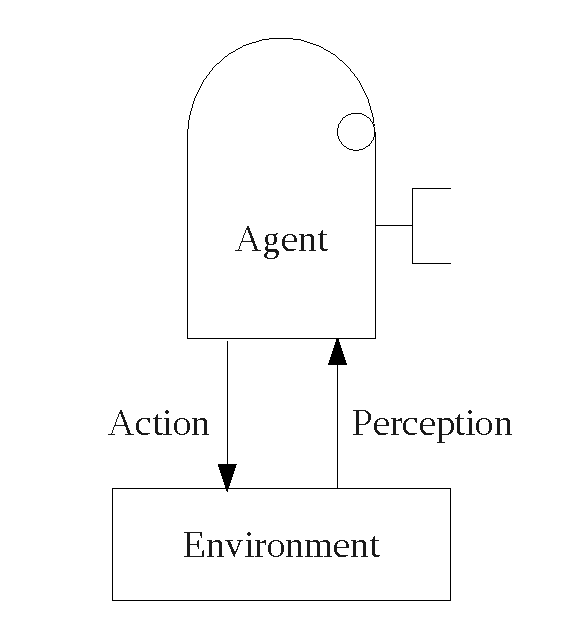
\includegraphics[height=5cm]{gfx/agent_environment}
  \caption[The agent environment model]{The agent environment model.}
  \label{fig:agent_environment}
\end{figure}

Figure~\ref{fig:agent_environment} shows the basic agent environment
model.  In this model, we make a distinction between the environment
and the agent.  At any given time, the agent and the environment are
each represented as a specific static form of data.  Further, these
representations change over time, according to a given transfer
function.  We will treat this system as a deterministic system,
although one could imagine adding random variables to the transfer
function: the basic theory is the same.  It is easier to add
randomness to a deterministic theory than the opposite.  There are
also many benefits to developing a deterministic model with perhaps a
pseudorandom aspect because this allows for the repeatability of
scientific experiments, for which the model may be used as a metric.
The two processes communicate information along two channels: (1) an
action channel from the agent to the environment, and (2) a perception
channel from the environment to the agent.


\section{The State-Action Model}

\begin{figure}[bth]
  \center
  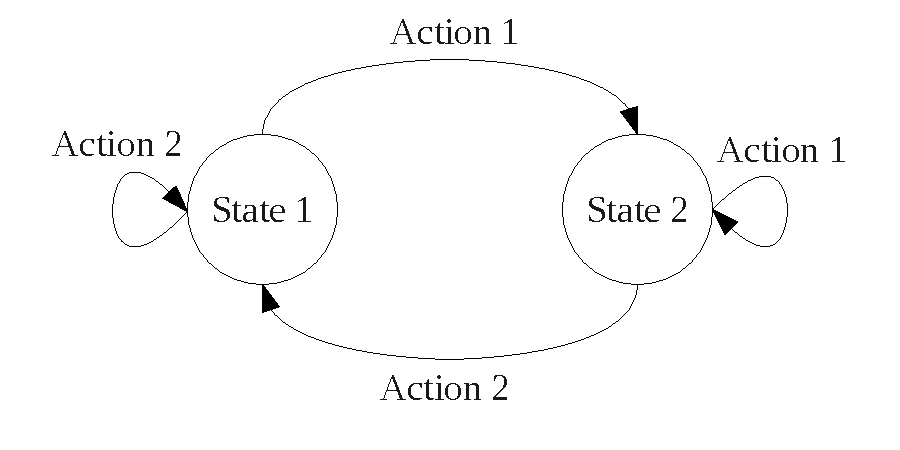
\includegraphics[width=6cm]{gfx/state_action}
  \caption[The state-action model]{The state action model.  Two states
    are represented by nodes and two actions are represented by edges
    from each of the two states.}
  \label{fig:state_action}
\end{figure}

The agent is in an environment, which is in a specific state.  Our
agent performs an action, which can affect the state of the
environment.  Figure~\ref{fig:state_action} shows a simple \ac{FSM}
state-action model, which has two states for the environment and two
actions for the agent to perform in each of these states.  The
state-action model is a simple model for how actions map to changes in
the state of the environment.

\section{Relational Representations as an Abstraction over State Spaces}

\begin{figure}[bth]
  \center
  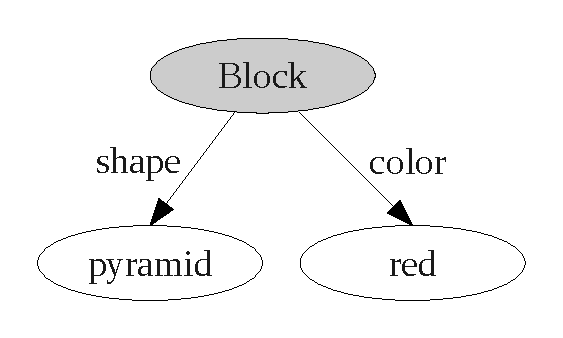
\includegraphics[height=3cm]{gfx/frame_representation}
  \caption[Frame-based relational representation.]{Frame-based relational representation.}
  \label{fig:frame_representation}
\end{figure}

See Figure~\ref{fig:frame_representation}.


\section{Frame Perceptions}

\begin{figure}[bth]
  \center
  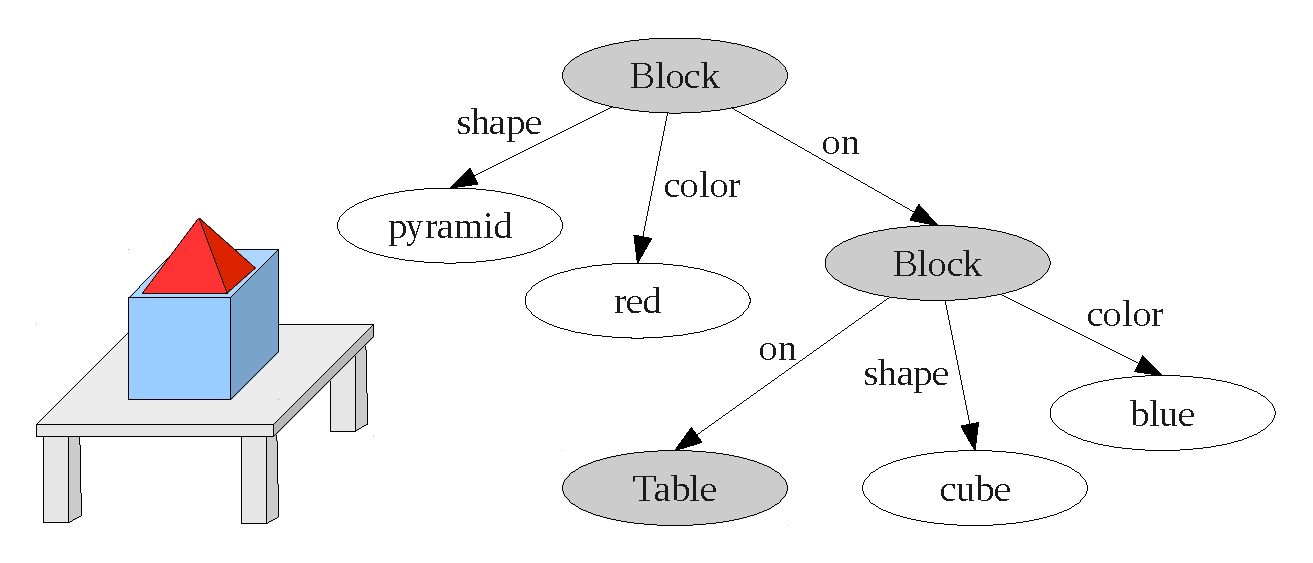
\includegraphics[height=5cm]{gfx/frame_perception}
  \caption[Collections of frames used as perceptual input to agent.]{Collections of frames used as perceptual input to agent.}
  \label{fig:frame_perception}
\end{figure}

See Figure~\ref{fig:frame_perception}.


\section{Partially Observable State Model}

\begin{figure}[bth]
  \center
  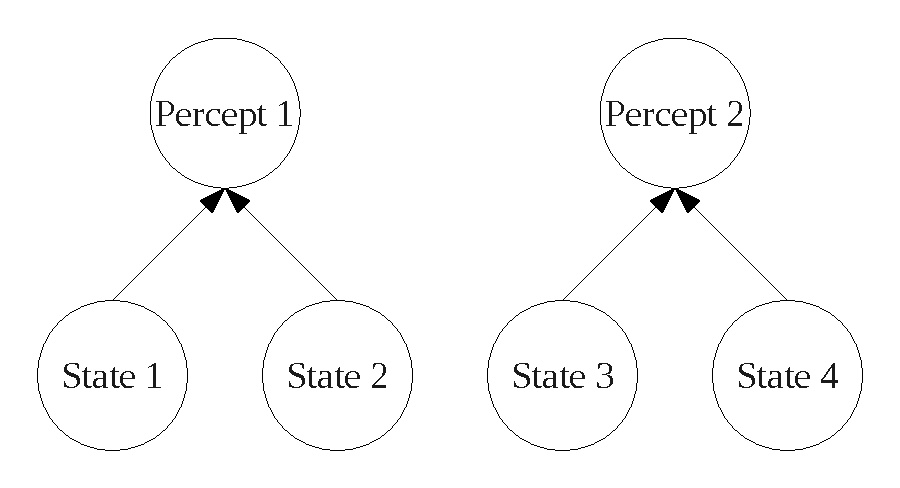
\includegraphics[width=6cm]{gfx/partially_observable}
  \caption[The partially observable state model]{The partially observable model.}
  \label{fig:partially_observable}
\end{figure}

The agent process does not have complete access to the state of its
environment.  The agent's perceptual stream of information depends on
the state of the environment, but it is a function of the environment
and not the actual state of the environment.  In other words, the
perceptual state that is communicated from the environment to the
agent is an injective function mapping the environment to the
perception of the agent.


\section{Partial Frame Perceptions}

\begin{figure}[bth]
  \center
  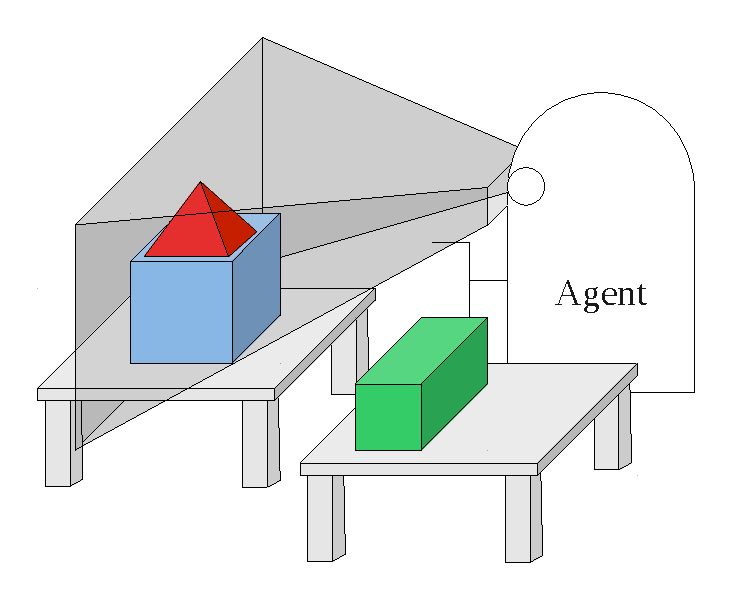
\includegraphics[height=5cm]{gfx/partial_frame_perception}
  \caption[The state of the environment is only partially observable.]{The state of the environment is only partially observable.}
  \label{fig:partial_frame_perception}
\end{figure}

See Figure~\ref{fig:partial_frame_perception}.


\section{Agent Abstract Physical Model}

\begin{figure}[bth]
  \center
  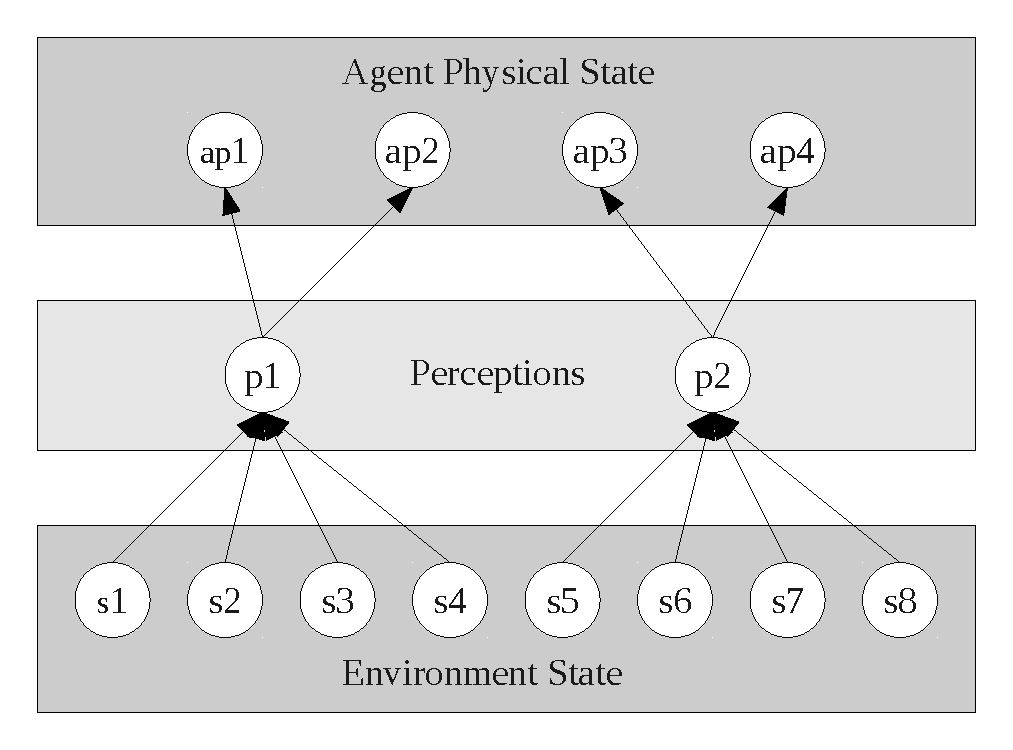
\includegraphics[width=8cm]{gfx/environment_perception_physical}
  \caption[The agent has an abstract physical model of the environment.]{The agent has an abstract physical model of the environment.}
  \label{fig:environment_perception_physical}
\end{figure}

See Figure~\ref{fig:environment_perception_physical}.


\section{A Physical Goal Representation}

\begin{figure}[bth]
  \center
  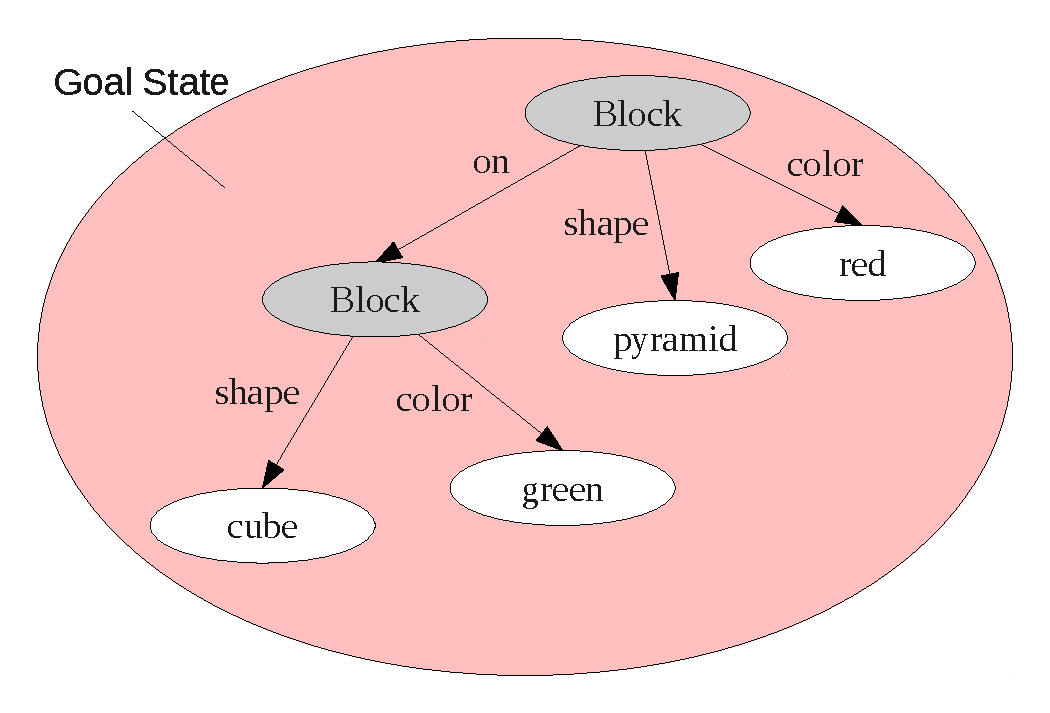
\includegraphics[height=4cm]{gfx/goal_state}
  \caption[A physical goal representation]{A physical goal representation is a structural relationship that may or may not currently exist within the physical knowledge base.}
  \label{fig:goal_state}
\end{figure}

See Figure~\ref{fig:goal_state}.


\section{The Multiple Agent Environment Model}

\begin{figure}[bth]
  \center
  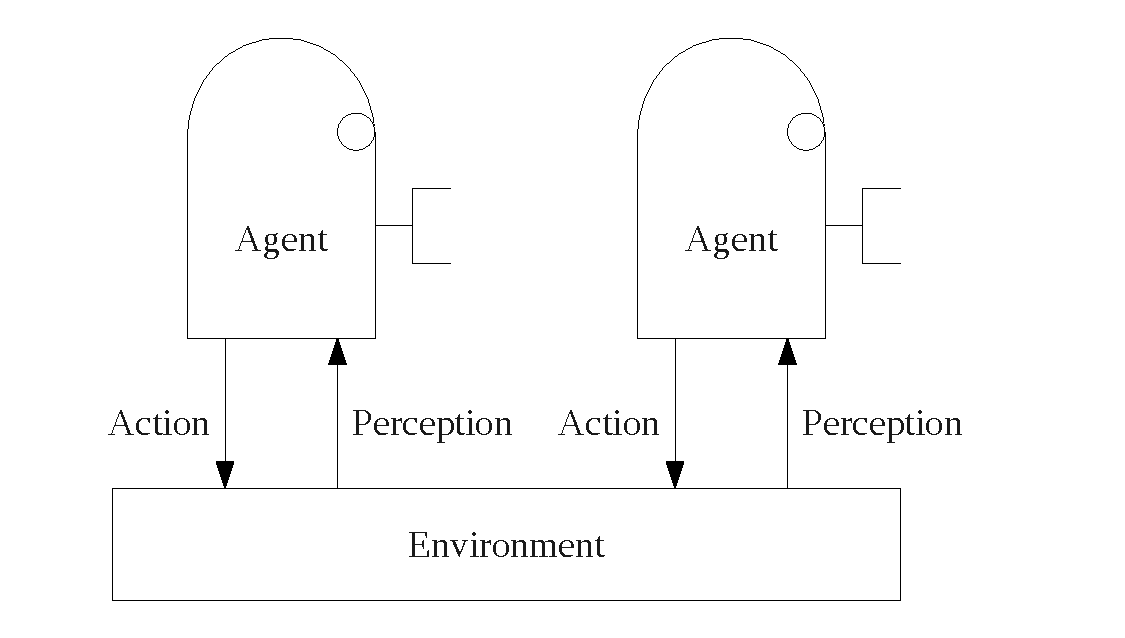
\includegraphics[height=5cm]{gfx/multiple_agent_environment}
  \caption[The multiple agent environment model]{The multiple agent environment model.}
  \label{fig:multiple_agent_environment}
\end{figure}

In order to model social intelligence, we introduce the multiple agent
environment model shown in
Figure~\ref{fig:multiple_agent_environment}.


\section{Agent Communication}

Because agent processes can only directly act on and perceive the
environment, all communication between agent processes must occur
through the environment process.  We assume that agents can
communicate some form of symbolic knowledge structure in the absence
of noise.  An example representation of a process is shown in


\begin{figure}[bth]
  \center
  {\hbox{
    \tt{[prog [pick-up knife]}
      
    \tt{~~~~~~[pick-up knife]]}
  }}
  
  \caption[Agent communication]{Agent communication.}
  \label{fig:agent_communication}
\end{figure}

